\chapter{Steer dynamics}
In the Whipple bicycle model, the steering wheel is modeled as a simple frictionless 1DoF rotational joint. In practice the dynamic behavior of this joint is expected to be more complex, for example; viscoses damping may be present due to air damping and Coulomb friction may occur due to friction caused by the bearings. Also some backlash is is observed, which is probably caused by the  torque limiter. The described effects may cause additional steering torques, which are not caused by the rider action. For rider identification, it is important to separate the system dynamics from the rider action. Therefore, the goal of this analysis is to quantify the dynamic properties of the steering joint.
\section{Experiment}
An simple experiment is set up to investigate the dynamic properties of the steering column. 2 springs are attached to the steer to create a known steering torque input, effectively creating a simple spring, mass and damper system. The small angle approximation of the torque caused by the 2 springs is given by:
		\begin{align}
		T_k = 2ek(\delta-\delta_0)
		\end{align}
Where $e$ represents the length of the moment arm, $k$ represents the spring stiffness and $\delta$ represents the angle. The steering angle $\delta$ is measured by using a pod meter. The steering rate is obtained by finite differencing of the steering angle. The rear frame of the bike is fixed to the external world and is assumed not moving at all. The measured parameters of the set up are shown in table \ref{table:measureparms}. Figure \ref{fig:example} shows a typical measurement. Here the steerangle is first set into a unstable position, before it is released at $t=\approx0.8$ [s]. The steer oscilates until it reaches its equilibrium position. 6 Measurements are peformed, consisting of 3 left and 3 right releases. A suitable datarange is selected by making use of the energy aproximation which corresponds to the desired small angle of 0.1 rad in combination with a fixed number of sucseeding datapoints.
\subsection{Calculating spring stiffnes}
The spring stiffness is determined by suspending the spring vertically and measure its length before and after a known amount of mass is added. The following spring stiffness is obtained.
\begin{align}
		k = \frac{\Delta F}{\Delta l} = \frac{g\Delta m}{l_2-l_1} = 912.77 \pm 66 \ \ \textrm{[N/m]}
\end{align}
\subsection{Data selection}
A suitable range of data is chosen based on the estimated energy of the system. The total energy of the system is decreasing because of the dissipation of energy caused by viscous damping and Coulomb friction. When the energy level exceeds a certain tress-hold (corresponding with the potential energy equal to 0.1 rad) the first data point is selected. Secondly, a fixed number of succeeding data-points is selected to complete the datarange. The selection method is shown in figure \ref{fig:energysel} and the resulting dataset for all six measurements is shown in figure \ref{fig:deltasel}. 
		\begin{table}
				\centering
				\begin{tabular}{cccl}
				\toprule
				Symbol & Value & Units & Description \\
				\midrule
				$l_1$ 	& $0.165\pm0.002$ & [m] & spring length 1 \\
				$l_2$ 	& $0.204\pm0.002$ & [m] & spring length 2 \\
				$\Delta m$ 	& $3.628$ & [kg] & added mass \\
				$e$ 		& $0.231\pm0.003$  & [m]	& moment arm \\
				\bottomrule
				\end{tabular}
				\caption{}
				\label{table:measureparms}
		\end{table}		
		\begin{figure}
			\centering
				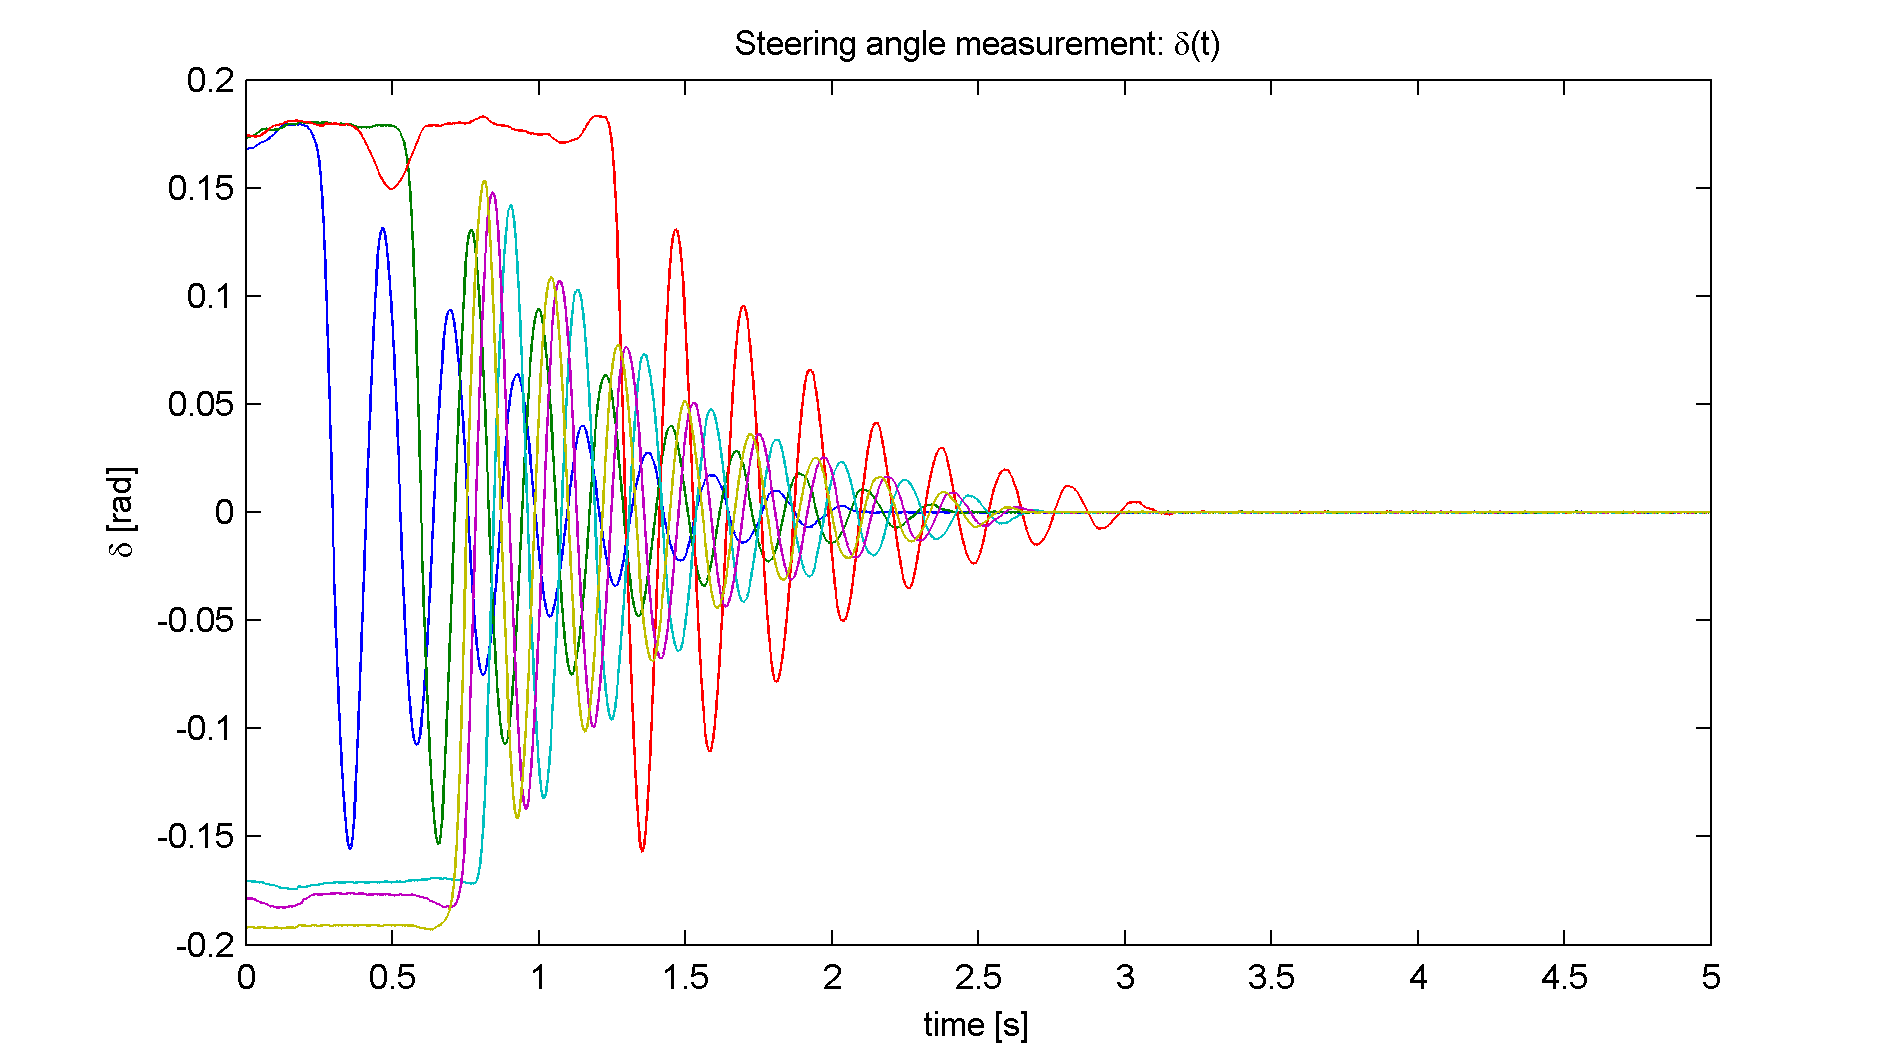
\includegraphics{images/example}
				\caption{}
				\label{fig:example}
		\end{figure}
		\begin{figure}
			\centering
				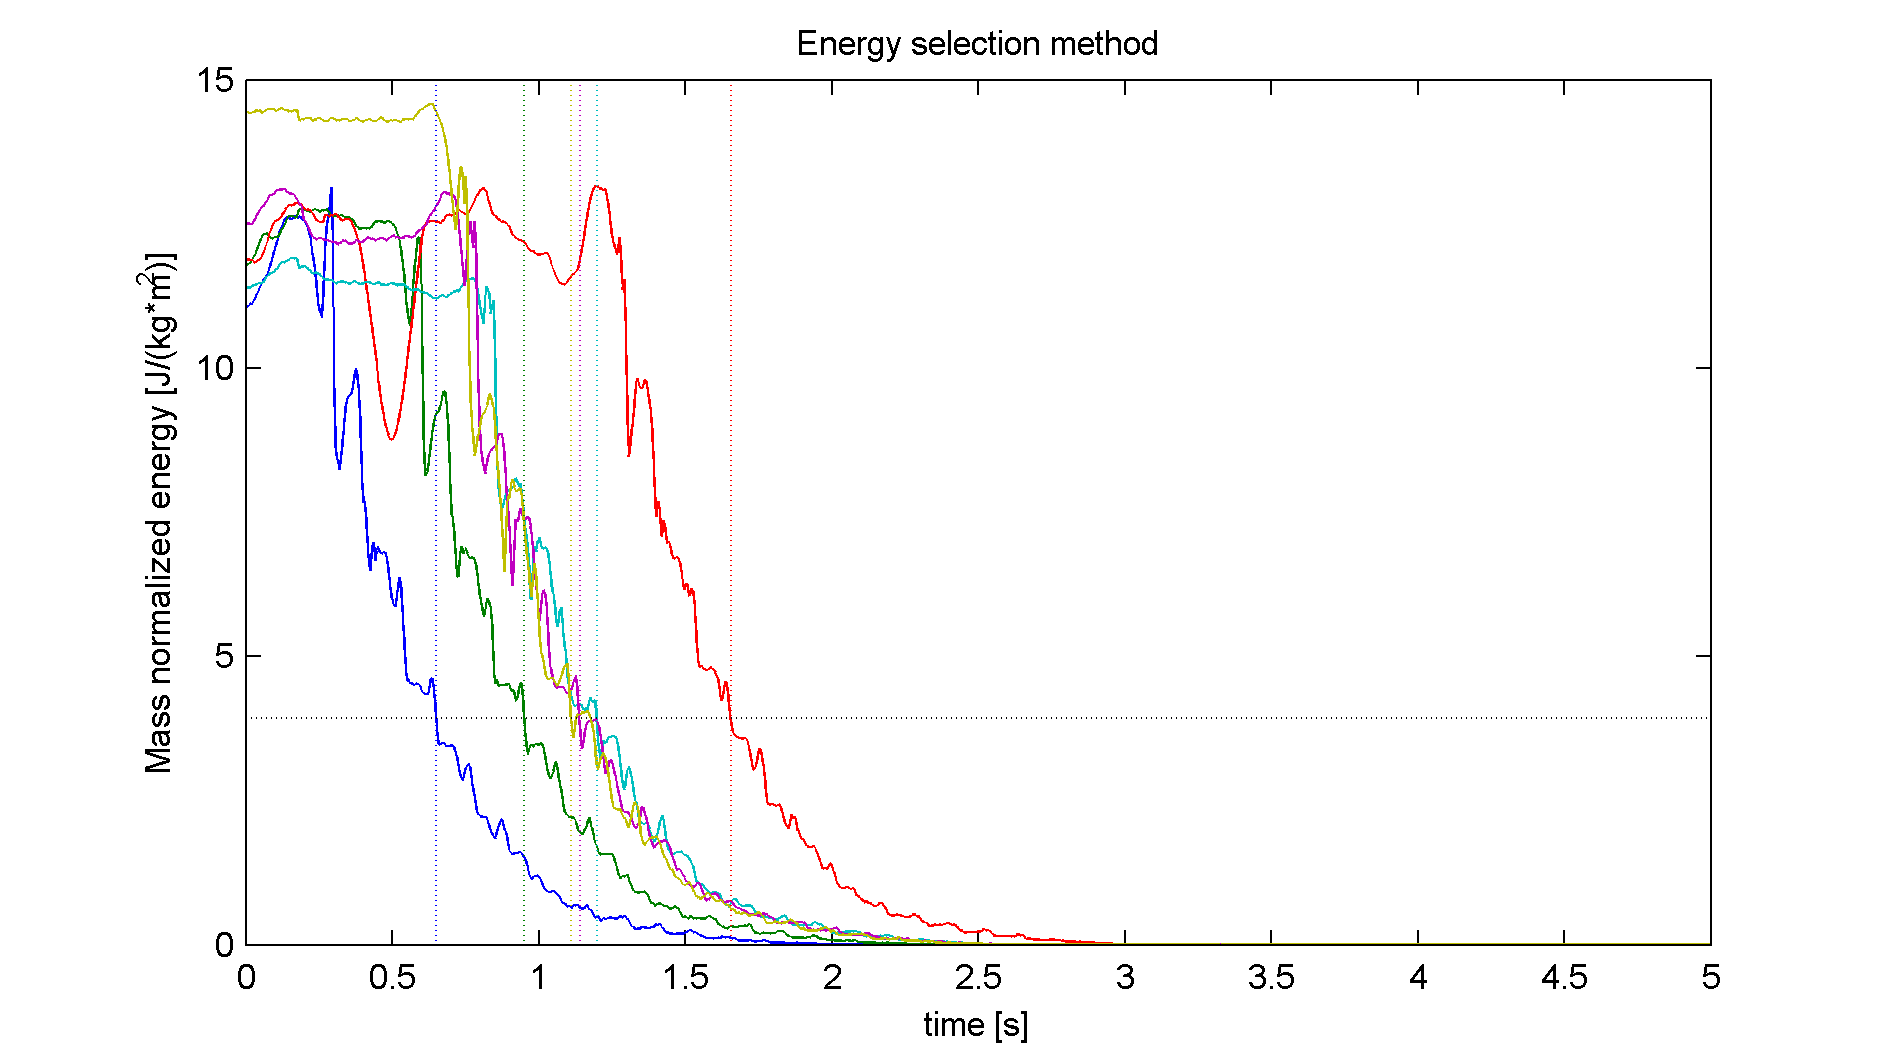
\includegraphics{images/energysel}
				\caption{Datarange selection based on estimated energy. The horizontal line represents the energy tresshold. The vertical lines represent the crossings of the tresshold values, which will be used as the first datapoint. Secondly a fixed range of sucseeding datapoint is selected to complete the selection.}
				\label{fig:energysel}
		\end{figure}
		\begin{figure}
			\centering
				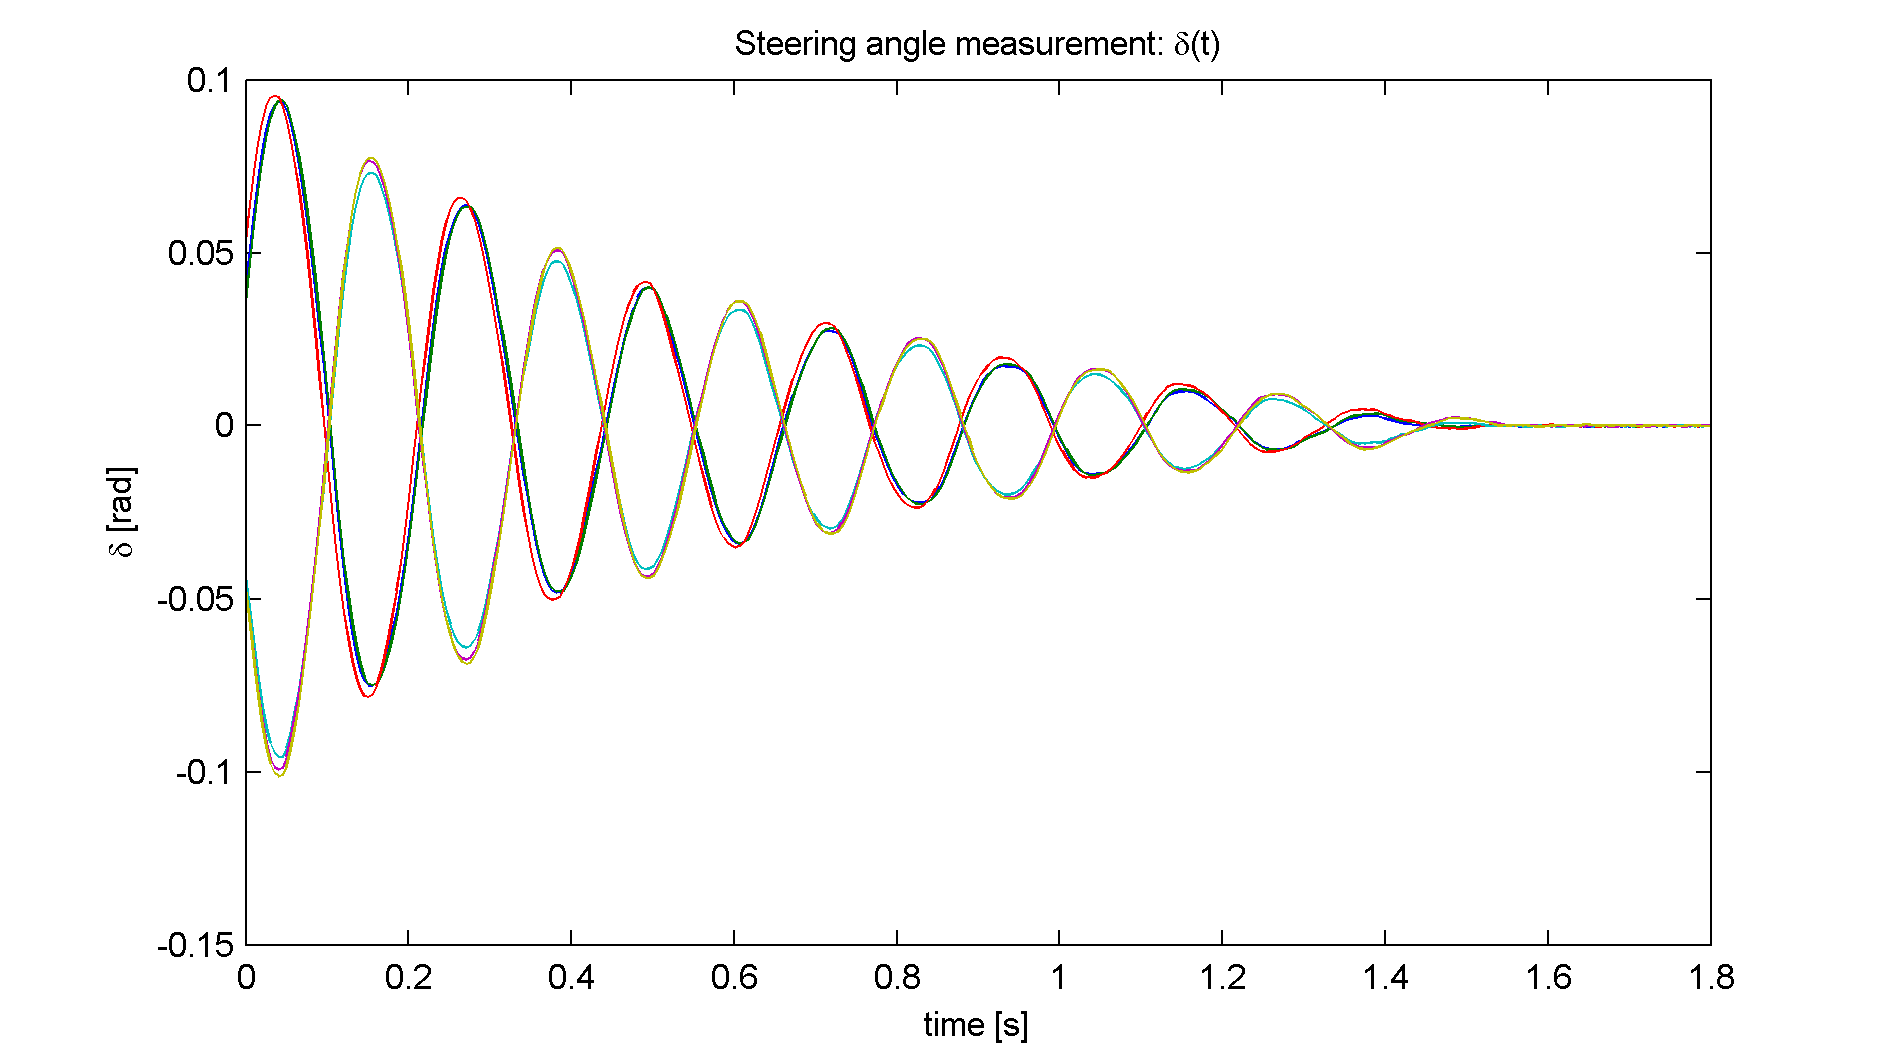
\includegraphics{images/deltasel}
				\caption{Selected datasets}
				\label{fig:deltasel}
		\end{figure}
\section{Model}
The dynamics of the font axis are modeled as a spring/mass/damper system with added Coulomb friction:
		\begin{align}
		\ddot{\delta} + 2\omega_0\zeta\dot{\delta} + \omega_0^2\delta =\tilde{F_c} 
		\end{align}
Where the Coulomb friction $\tilde{F_c} = \frac{F_c}{I_{\delta\delta}}$ is modeled as:
		\begin{align}
		\tilde{F}_c &= \left\{
				\begin{array}{rl}
				 A & \text{if } \dot{\delta} < 0,\\
				0 & \text{if } \dot{\delta} = 0 ,\\
							-A & \text{if } \dot{\delta} > 0.
				\end{array} \right.
		\end{align}
The Coulomb friction introduces an non-linear term in the differential equations. A time series solution of the non linear equations is obtained using the Matlab ODE45 solver. The unknown parameters $\zeta$, $\omega_0$ and $A$ are obtained from the experimental data by using parameter estiamation techniques. Here a Levenberg Marquad algorithm is used for estimating the parameters. 
\section{Results}
The identification algorithm is repeated for 6 measurements. The resulting parameters are shown in the table below: 
%		\begin{table}
				\begin{center} 
				\begin{tabular}{cccc}
				\toprule
				$n$ & $\omega_0$ & $\zeta$ & $A$ \\
				\midrule
				1  & 27.7347  &  0.0455  &  0.9963\\
				2	& 27.7179  &  0.0493  &  0.7559\\
				3	& 27.7228  &  0.0539  &  0.7166\\
				4	& 27.6573  &  0.0505  &  0.7078\\
				5	& 27.5571  &  0.0307  &  1.6129\\
				6	& 27.5462  &  0.0533  &  0.5515\\
				\bottomrule
				\end{tabular}
				\end{center}
The resulting fits are shown in figure \ref{fig:fitting}. Since both the eigenfrequency and stifness are known, a estimate of the mass moment of inertia can be made:
\begin{align}
\omega_0^2 = \frac{2ke}{I_{\delta\delta}}  \ \Rightarrow \  I_{\delta\delta} = \frac{2ke}{\omega_0^2} = 0.55\pm0.04 \ \textrm{[kg/m$^2$]}
\end{align}
%				\caption{}
%				\label{table:parms}
%		\end{table}
		\begin{figure}
			\centering
				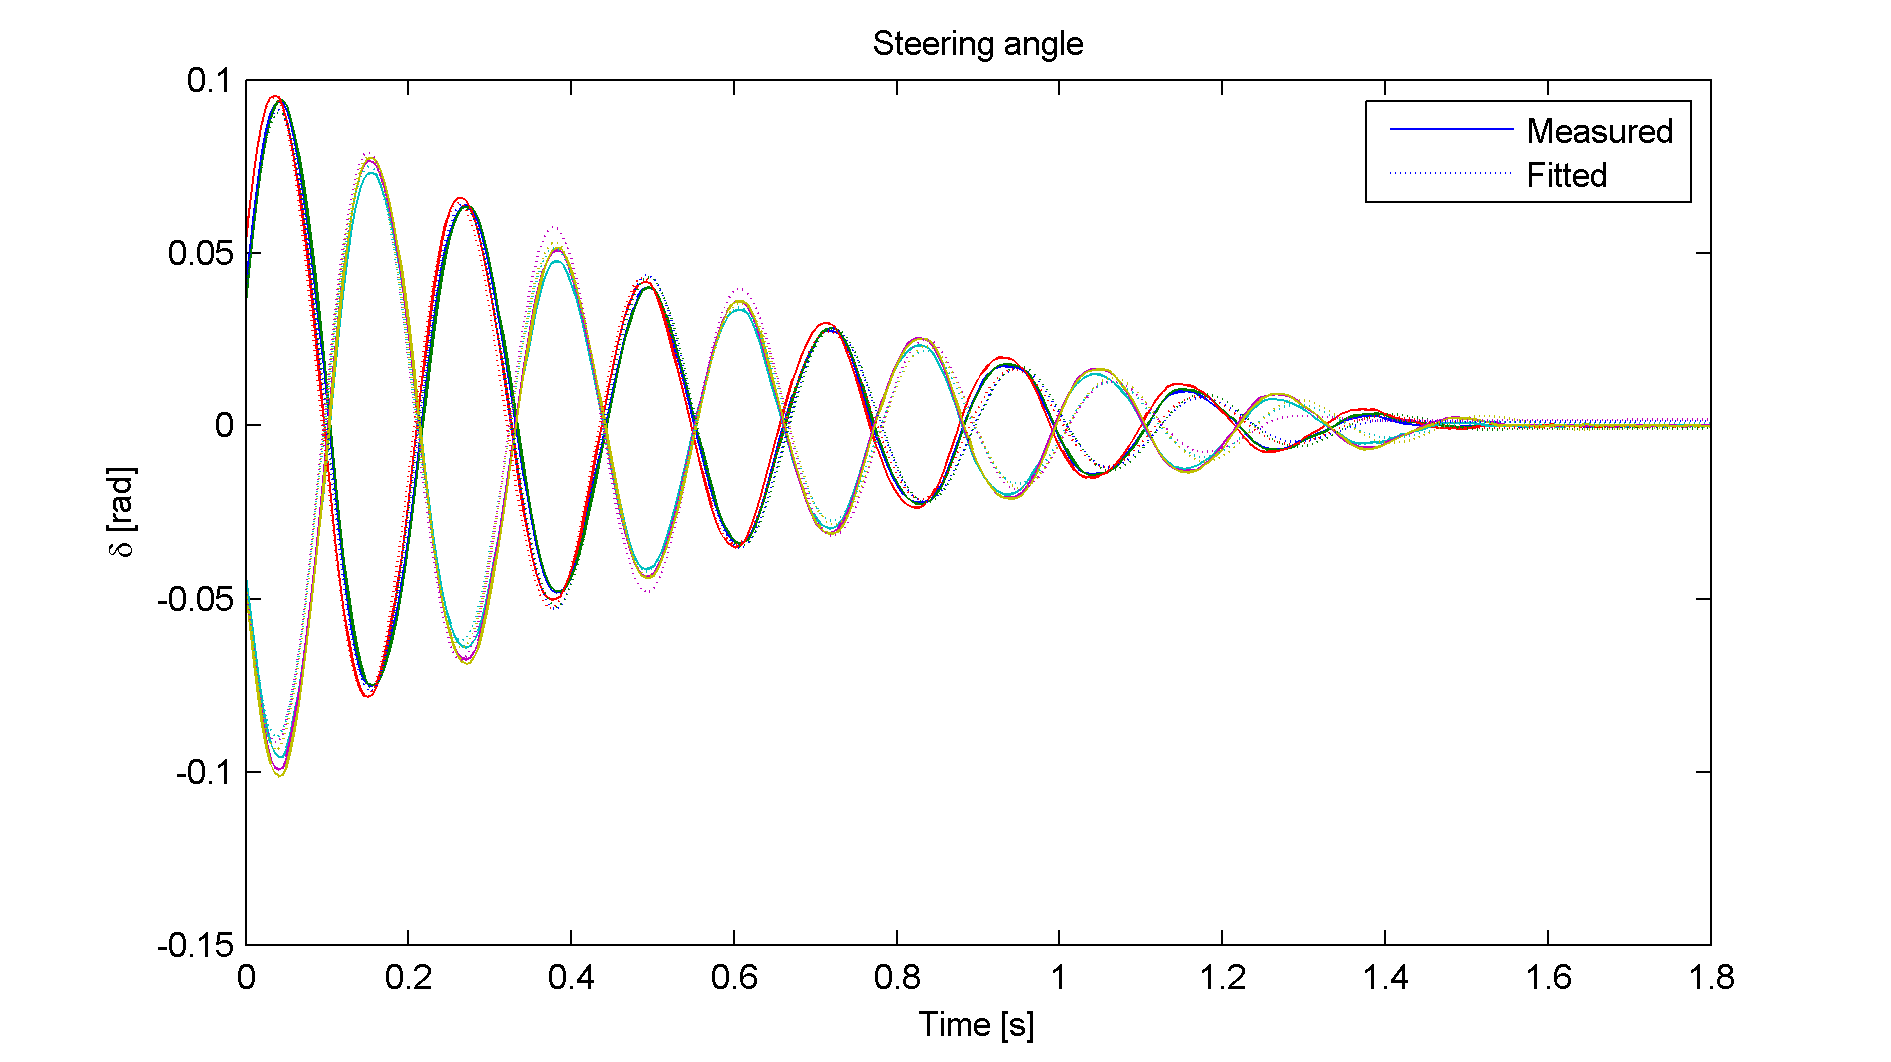
\includegraphics{images/fitting}
				\caption{}
				\label{fig:fitting}
		\end{figure}
\section{Application}
To get an idea of the relative influence of the damping on the steering torque measurements, the damping model is applied to some of the actual measurements. First the damping equations are rewritten to obtain the damping torque $F_d$.
		\begin{align}
		F_d =  {F_c}  -  2\omega_0\zeta I_{\delta\delta} \dot{\delta}
		\end{align}
The damping torque is then plotted together with the measured torque to get an idea of the relative amplitude. The result is shown in figure \ref{fig:torque}
		\begin{figure}
			\centering
				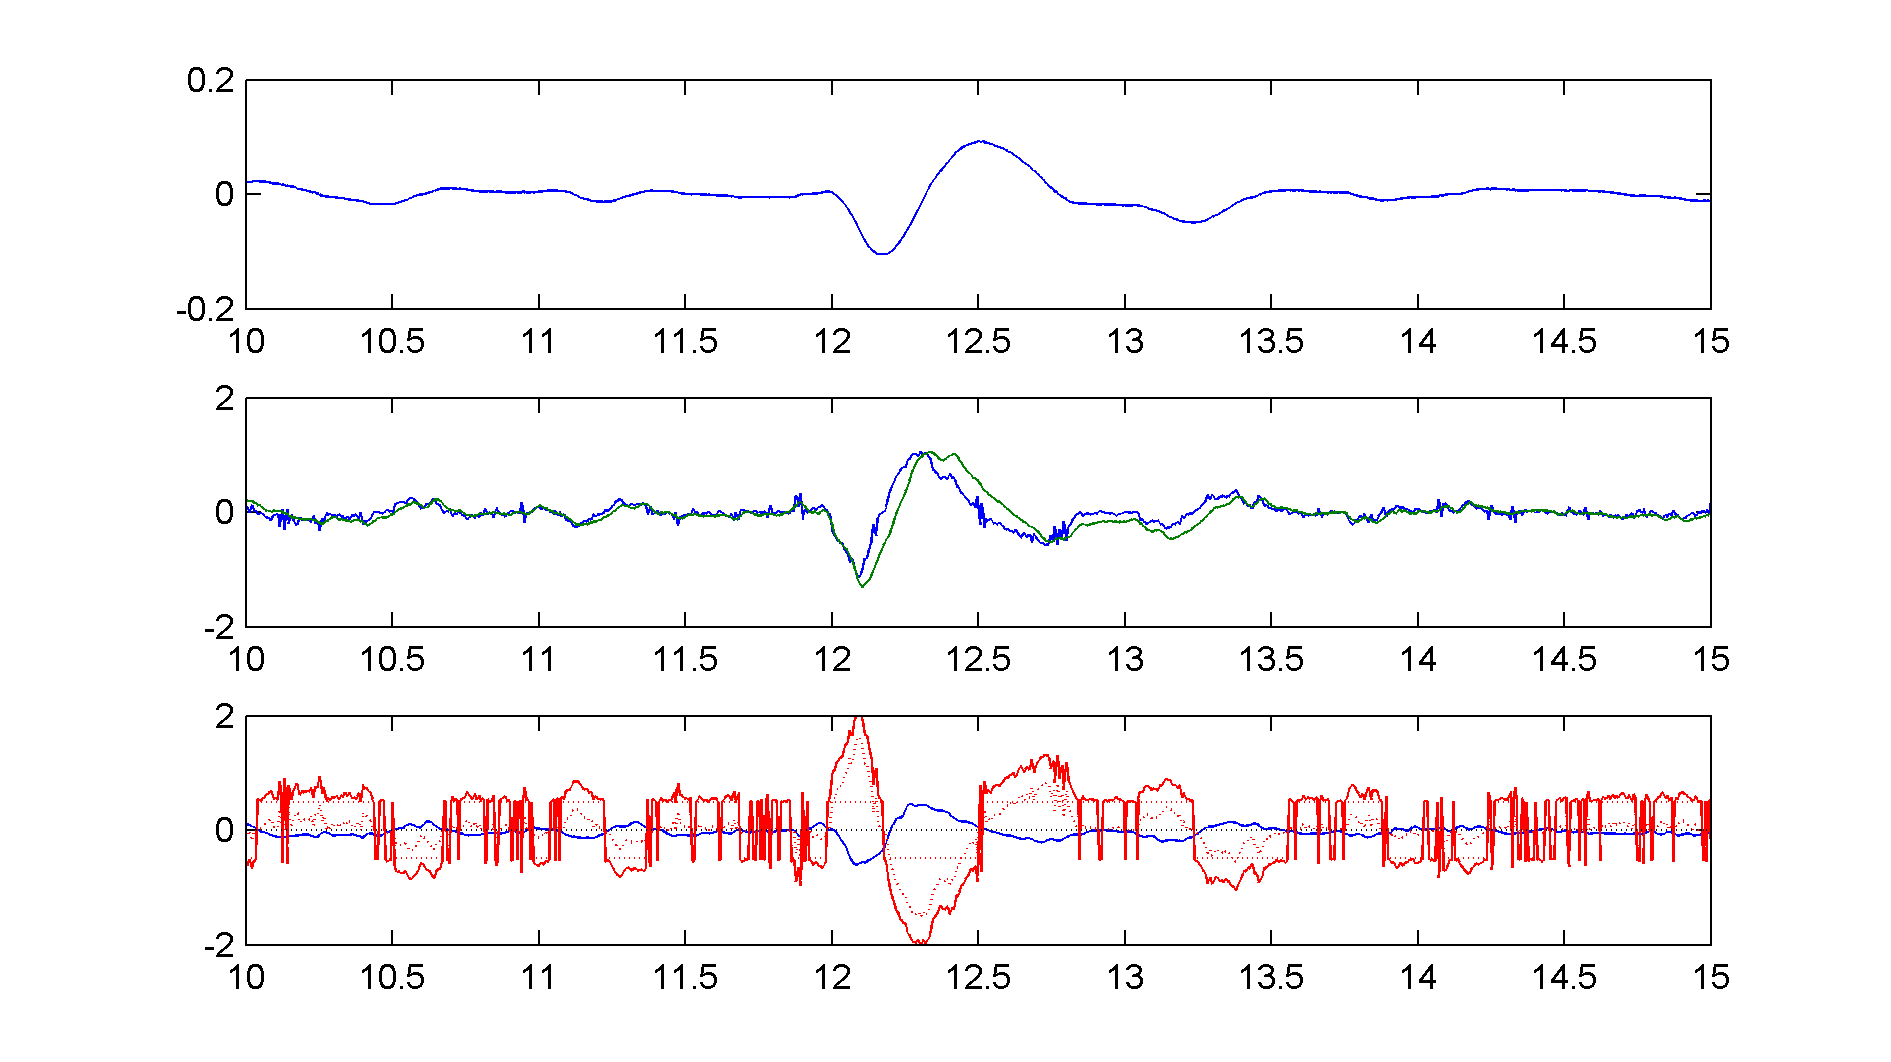
\includegraphics{images/torque}
				\caption{}
				\label{fig:torque}
		\end{figure}
\section{Discussion}
\begin{itemize}
\item Eigenfrequency very consistent
\item Both the Coulomb friction and viscous damping show relatively a lot of variation
\item System seems to be symmetric around $\delta_0$. 
\item Model fits amplitude very well
\item Model has trouble matching the phase.
\end{itemize}
\section{Conclusion}
		\begin{itemize}
				\item Total amount of friction seems to be significant and may not be omitted.
				\item Friction is consists of viscous damping and Coulomb friction.ous damping and Coulomb friction.
		\end{itemize}
\section{Future work} 
		\begin{itemize}
				\item Figure out backlash principle and model it mathematically, incorporate there results in the bike model.
				\item Apply friction model combined with separate inertia models to obtain rider steering torque. 
		\end{itemize}
\section{Some additional analysis}
Figure \ref{fig:steer1} and \ref{fig:steer2} show some additional analysis of the steer dynamics.
		\begin{figure}
			\centering
				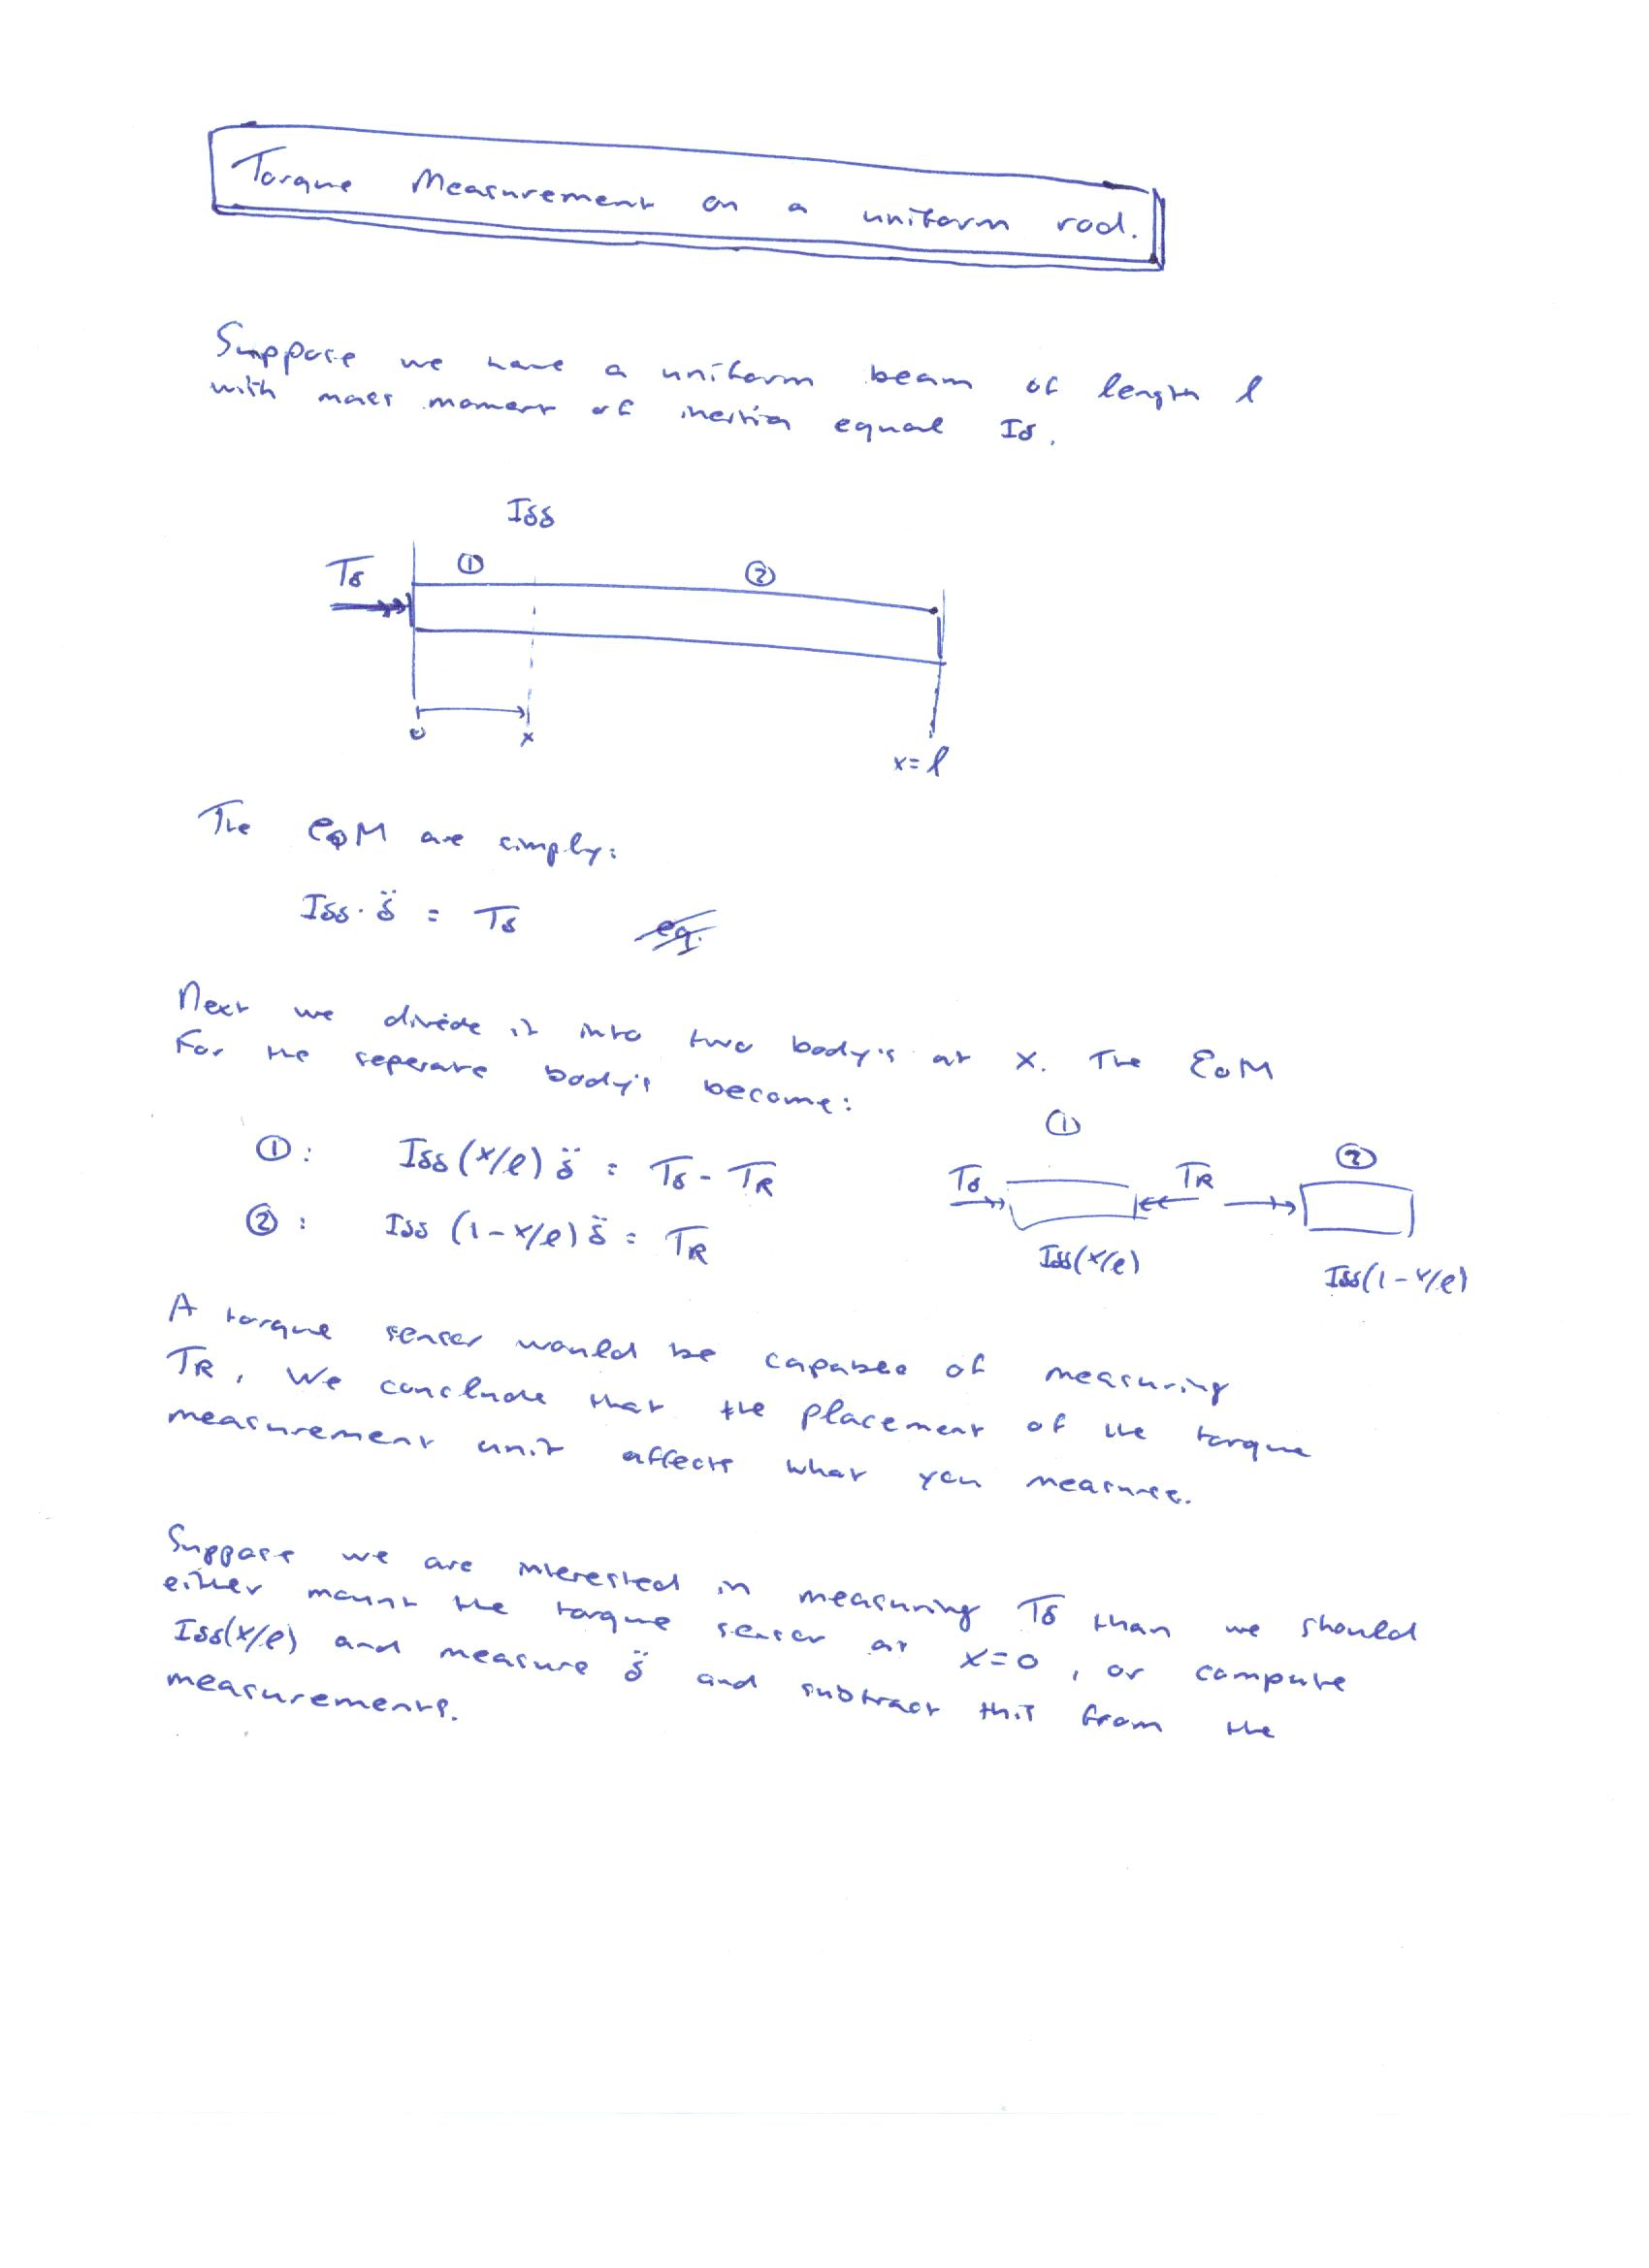
\includegraphics[width=16cm]{images/torquemeasurement.jpg}
				\caption{Torque measurement on uniform bar example}
				\label{fig:steer1}
		\end{figure}
		\begin{figure}
			\centering
				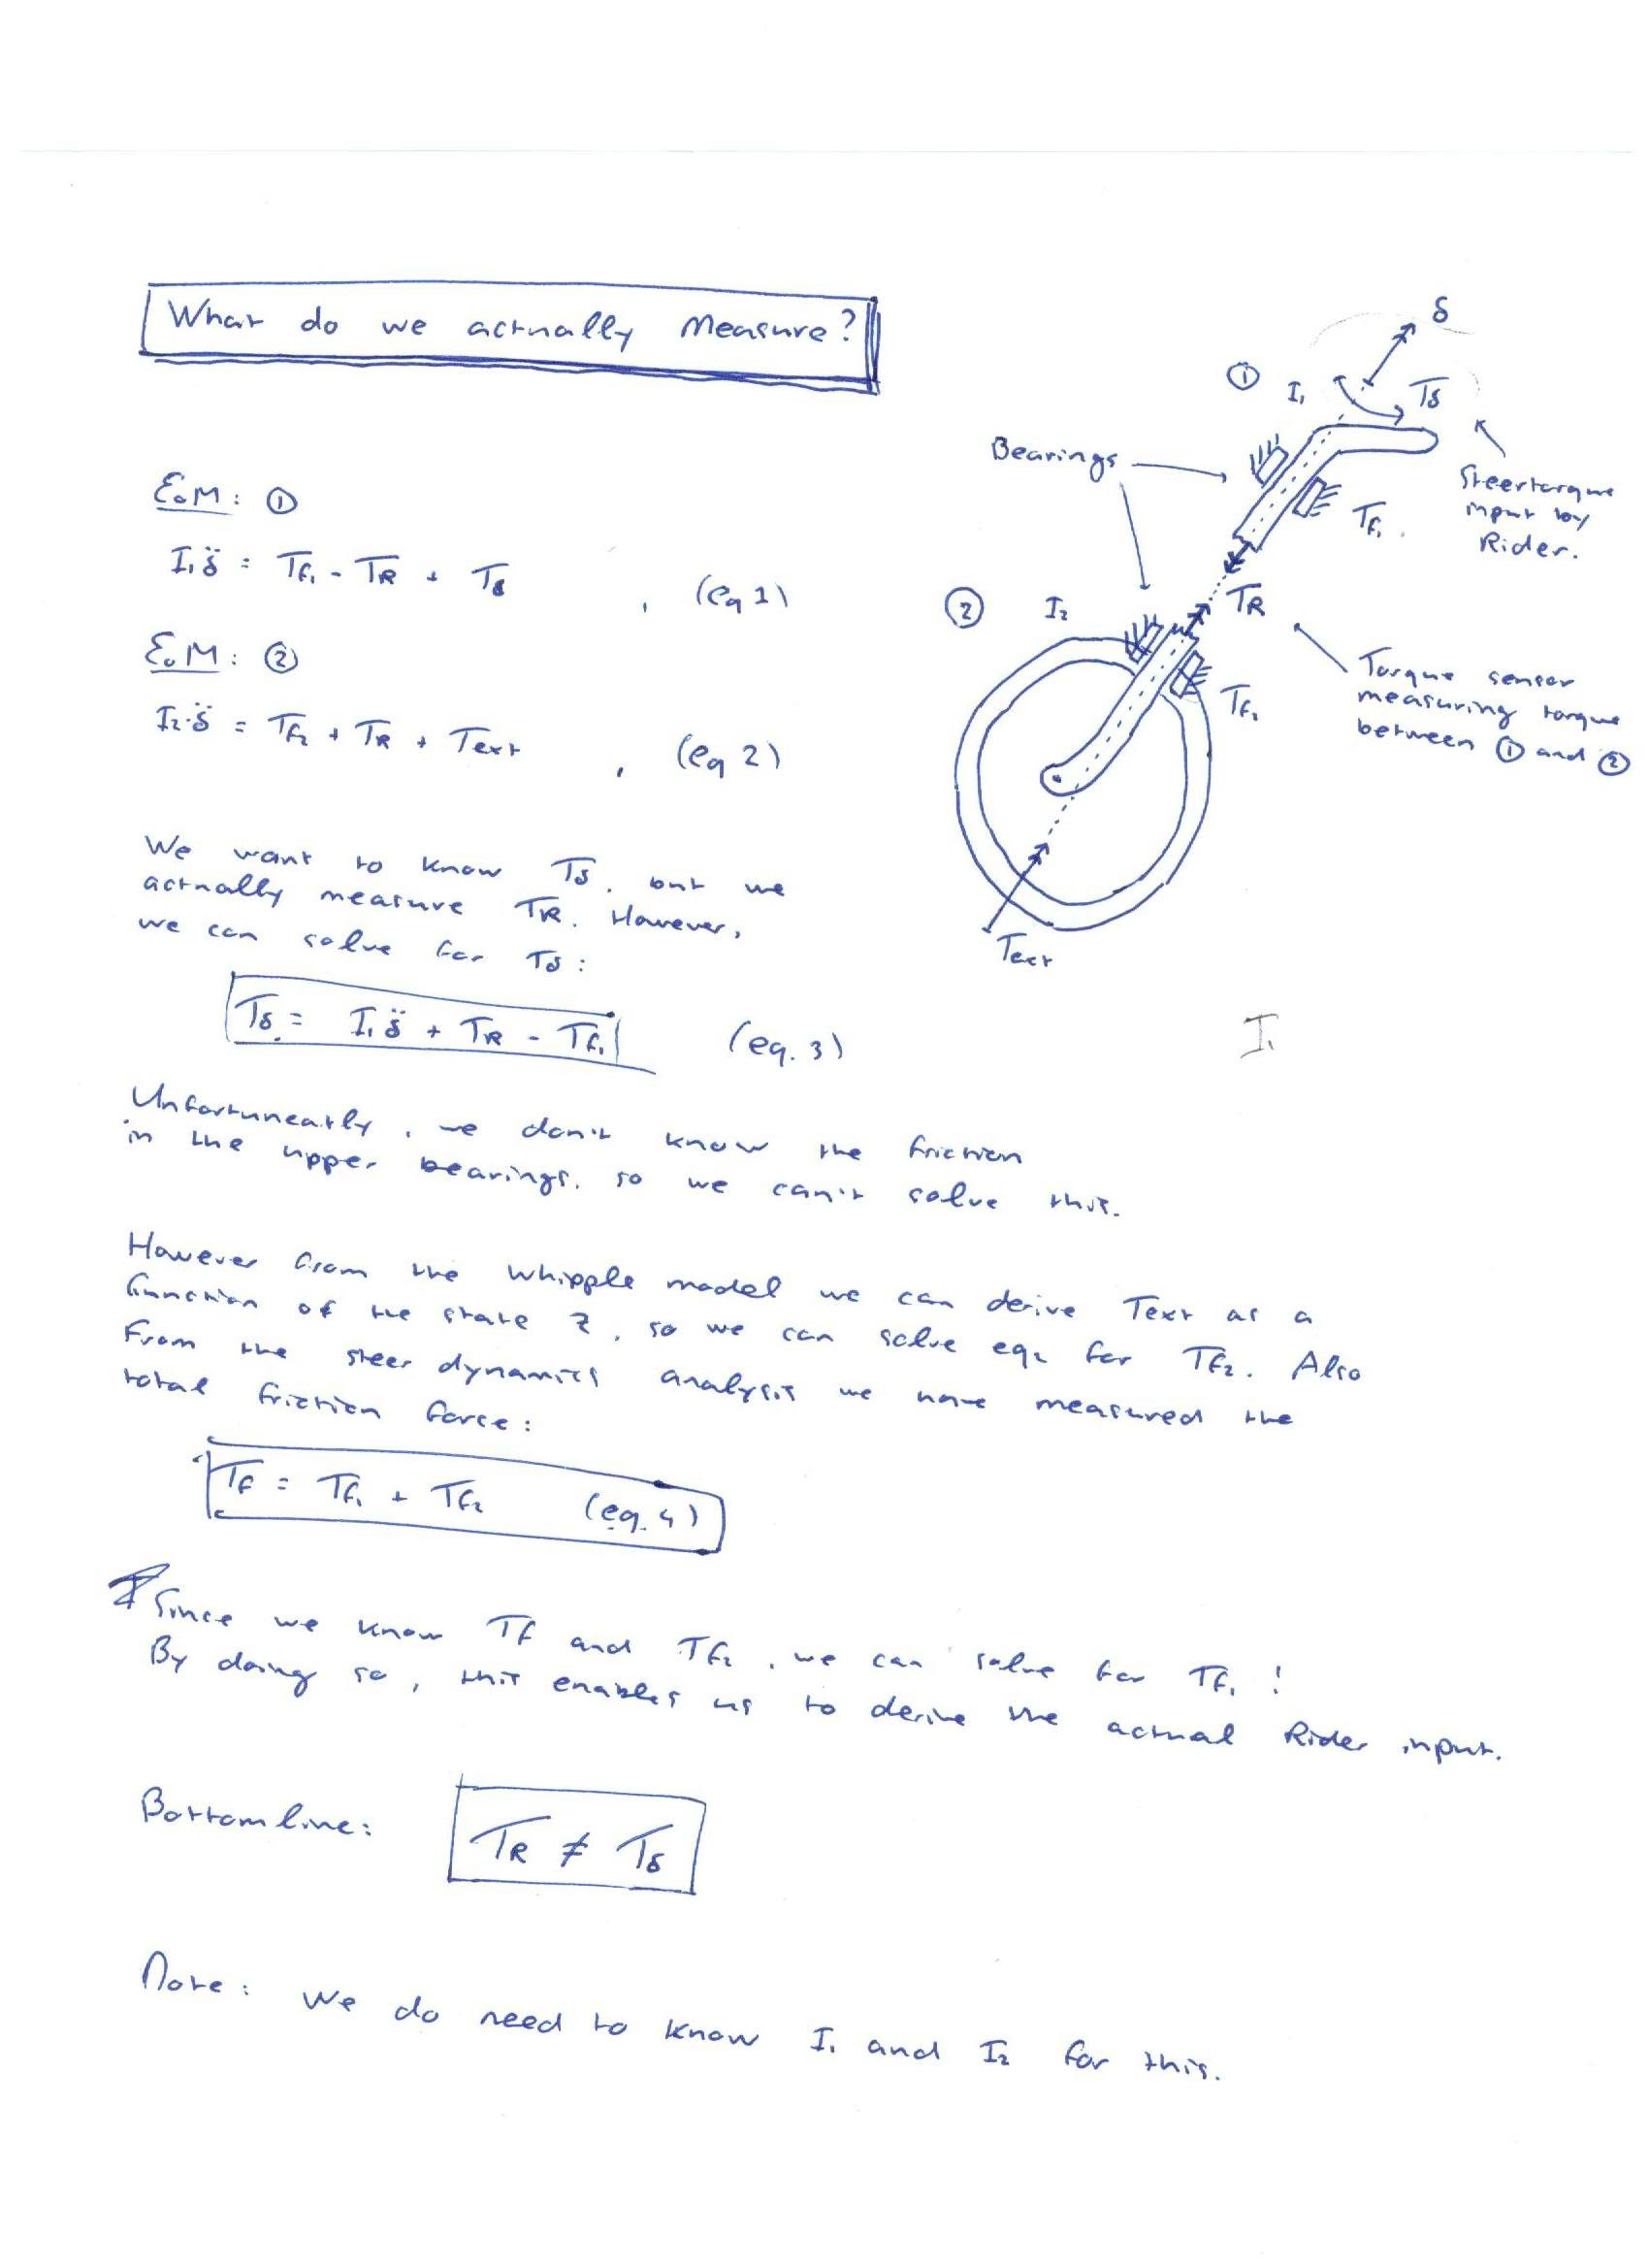
\includegraphics[width=16cm]{images/steeringequations.jpg}
				\caption{Equations of motion governing the steering dynamics}
				\label{fig:steer2}
		\end{figure}
\end{document}